\documentclass[12pt, a4paper]{scrreprt}
\usepackage[margin=2.5cm]{geometry}
\usepackage[hidelinks]{hyperref}
\usepackage{graphicx,xcolor,listings,tikz,enumitem}
\usetikzlibrary{positioning, arrows.meta, shapes, fit}

\definecolor{codegreen}{rgb}{0,0.6,0}
\definecolor{codegray}{rgb}{0.5,0.5,0.5}
\definecolor{codepurple}{rgb}{0.58,0,0.82}
\definecolor{backcolour}{rgb}{0.95,0.95,0.92}

\lstdefinestyle{mystyle}{
  backgroundcolor=\color{backcolour},
  commentstyle=\color{codegreen},
  keywordstyle=\color{blue},
  stringstyle=\color{codepurple},
  basicstyle=\ttfamily\footnotesize,
  numbers=left,
  numbersep=5pt,
  breaklines=true,
  tabsize=2
}
\lstset{style=mystyle}

\newcommand{\faculty}{Faculty Applied Information Technology}
\newcommand{\studies}{Bachelor of Cyber-Security}
\newcommand{\thesistitleDE}{Projekt "WeedDetector" - Eigenanteil Manuel Friedl}
\newcommand{\submissiondate}{05.\ Juli 2025}
\newcommand{\supervisor}{Prof.\ Dr.\ Holger Jehle}

\begin{document}

\begin{titlepage}
  \centering
  {\LARGE Technische Hochschule Deggendorf \\ \faculty \par}
  \vspace{0.3cm}
  {\Large Studiengang \studies \\[1.5cm]}
  {\Huge\bfseries \thesistitleDE\par}
  \vfill
  \begin{minipage}[t]{0.45\textwidth}
    \textbf{Vorgelegt von:}\\
    \\
    Manuel Friedl (12306626)\\
    \\
    \\
    \\
    \\
    Datum: \submissiondate
  \end{minipage}\hfill
  \begin{minipage}[t]{0.45\textwidth}
    \textbf{Prüfungsleitung:}\\
    \\
    \supervisor
  \end{minipage}
\end{titlepage}

\tableofcontents
\newpage

\chapter{Einleitung}
In diesem Abschnitt wird mein persönlicher Beitrag zum Projekt \textbf{"Weed Detector“} im Rahmen des Software Engineering Kurses dargestellt. Ziel ist es, die von mir übernommenen Aufgaben sowie meinen Anteil an der Planung, Umsetzung und Optimierung des Projekts transparent zu machen.\\
\\
Dabei werden sowohl die \textbf{technischen Aufgaben}, die ich im Verlauf des Projekts übernommen habe, als auch \textbf{meine Beiträge zur Zusammenarbeit im Team} beschrieben. So wird nachvollziehbar, welche Bereiche des Weed Detectors maßgeblich von mir entwickelt oder betreut wurden und wie mein Beitrag zur erfolgreichen Fertigstellung des Projekts beigetragen hat.

\chapter{Implementierung des Graphical User Interfaces}
Ein wesentlicher Teil meines Beitrags war die Entwicklung und Implementierung der grafischen Benutzeroberfläche (GUI) für den Weed Detector unter Verwendung von Tkinter in Python.\\
\\
Bei der Umsetzung habe ich das MVC-Designpattern (Model-View-Controller) angewendet, um die Struktur und Wartbarkeit des Codes zu verbessern. Die View umfasst die Tkinter-Oberfläche mit den Steuerelementen und der Visualisierung der Unkrauterkennung. Die Controller-Logik verbindet die Benutzerinteraktionen mit der Modelllogik zur Bildanalyse und Steuerung der Demo-Funktionen, während das Model die Ergebnisverarbeitung und Steuerung der Detektion beinhaltet.

\section{Zentrale Aufgaben der GUI}
Die \textbf{GUI des Weed Detectors} übernimmt folgende zentrale Aufgaben:
\begin{itemize}
    \item \textbf{Bilddateien auswählen:} Ermöglicht das Laden von gespeicherten Bildern zur Analyse durch das YOLOv8-Modell.
    \item \textbf{Live-Kamera starten:} Aktiviert die integrierte oder angeschlossene Kamera zur Echtzeiterkennung von Unkraut.
    \item \textbf{Roboter-Demo starten:} Startet die simulierte Roboterbewegung auf einer vordefinierten Strecke zur Demonstration des automatisierten Erkennungs- und Bekämpfungsprozesses.
    \item \textbf{Visualisierung der Ergebnisse:} Zeigt die Erkennungsergebnisse direkt in der GUI an, indem erkannte Unkräuter markiert und hervorgehoben werden.
    \item \textbf{Einfache Bedienung und Steuerung:} Bietet eine benutzerfreundliche Schnittstelle zur Steuerung des Weed Detectors ohne manuelle Eingriffe im Code.
    \item {Status- und Fortschrittsanzeige:} Informiert den Benutzer über den aktuellen Status von Analyse und Roboterbetrieb, um den Ablauf nachvollziehbar zu gestalten.
\end{itemize}
Diese Aufgaben ermöglichen eine effiziente und intuitive Nutzung des Weed Detectors, sodass alle Funktionen zentral zugänglich und die Ergebnisse der Unkrauterkennung leicht überprüfbar sind.

\newpage

\section{Prozess der GUI}
Nach der Anforderungsanalyse begann die Entwicklung der GUI zunächst mit einem einfachen Fenster und zwei Buttons (Bild hochladen, Live-Kamera starten) als ersten Prototypen, um eine funktionale Basis zu schaffen und die Kernfunktionen frühzeitig testen zu können.\\
\\
Im nächsten Schritt wurde die GUI vollständig refactored, um eine anspruchsvollere, optisch ansprechendere und nahtlose Benutzererfahrung zu ermöglichen. Dies umfasste die Anpassung des Layouts, eine verbesserte Strukturierung der Elemente sowie die Integration eines einheitlichen Designs.\\
\\
Anschließend wurde die GUI nach dem MVC-Designpattern umgebaut, um die Struktur und Wartbarkeit zu verbessern. Hierbei wurden Call-Back-Funktionen eingesetzt, um Benutzerinteraktionen effizient mit der Verarbeitungslogik und Ergebnisanzeige zu verbinden.\\
\\
Die Ergebnisse der Unkrauterkennung werden nun sowohl visuell im Kamerafenster als auch in einem Result Panel angezeigt, während Aktionen des simulierten Roboters in einem Roboter Status Panel ausgegeben werden, sodass der Nutzer den gesamten Prozess nachvollziehen kann.\\
\\
Zum Abschluss wurden Tests geschrieben und Optimierungen durchgeführt, um die Stabilität, Performance und Benutzerfreundlichkeit der GUI sicherzustellen.\\

\subsection{Callbacks in der GUI}
In der Tkinter-GUI werden Callbacks verwendet, um Benutzeraktionen mit Funktionen zu verknüpfen. Ein Callback ist dabei eine Funktion, die automatisch ausgeführt wird, sobald der Benutzer eine bestimmte Aktion ausführt, wie z.B. das Klicken eines Buttons.\\
\\
\begin{lstlisting}[language=Python, caption=Callback-Definition]
    self.on_select_image = None # Callback for image selection
    self.on_detect = None # Callback for detection
    self.on_start_robot = None  # Callback for robot start
    self.on_stop_robot = None  # Callback for robot stop
    self.on_camera_frame = None # Callback for camera frame processing
\end{lstlisting}

\begin{lstlisting}[language=Python, caption=Beispiel Callback-Verwendung]
    ...
    if file_path and callable(self.on_select_image):
            self.on_select_image(file_path)
\end{lstlisting}

\begin{figure}[h!]
    \centering
    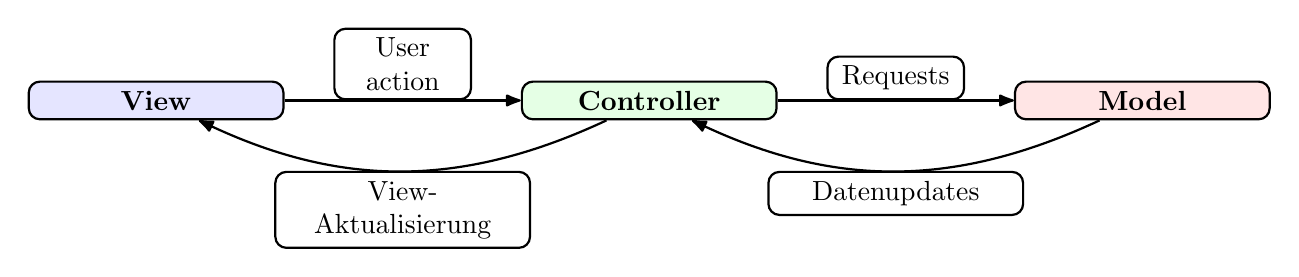
\begin{tikzpicture}[
        scale= 1.0,            % shrink everything to 70%
        transform shape,      % apply the scale to node shapes & text
        node distance=3 cm and 3cm,
        every node/.style={draw, text width=3cm, align=center, rounded corners},
        every path/.style={draw, thick, -{Latex[round]}}
    ]

    % Nodes
    \node (view) [fill=blue!10] {\textbf{View}\\};
    \node (controller) [right=of view, fill=green!10] {\textbf{Controller}\\};
    \node (model) [right=of controller, fill=red!10] {\textbf{Model}\\};

    % Arrows
  \path (view) -- node[above,text width=1.5cm]{User action} (controller);
  \path (controller) -- node[above,text width=1.5cm]{Requests} (model);
    \path (model) to[bend left=25] node[below]{Datenupdates} (controller);
    \path (controller) to[bend left=25] node[below]{View-Aktualisierung} (view);

    \end{tikzpicture}
    \caption{MVC-Architektur der WeedDetector-Anwendung}
    \label{fig:mvc-diagramm}
\end{figure}

\chapter{Roboter und Navigation}
Ein weiterer zentraler Beitrag von mir war die Implementierung des \emph{"Demo"}-Roboters, welcher den realen Einsatz eines Unkrauterkennungsroboters simuliert. Ziel war es, die Prozesskette von der Erkennung bis zur gezielten Bekämpfung in einer sicheren Testumgebung realistisch darzustellen.\\
\\
Hierfür wurde eine \textbf{Robot}-Klasse entwickelt, die folgende Kernfunktionen umfasst:
\begin{itemize}
    \item \textbf{start\_robot:} Startet den Roboter, aktiviert die Kamera und initiiert den Fahrprozess in einem eigenen Thread, sodass die GUI reaktiv bleibt.
    \item \textbf{stop\_robot:} Stoppt den Roboter und beendet den Fahrprozess sicher.
    \item \textbf{drive\_loop:} Führt den Fahrvorgang in einer Schleife aus, liest kontinuierlich Bilder von der Kamera ein, führt die Unkrauterkennung mit YOLOv8 durch und zeigt die Ergebnisse live in der GUI an. Wird Unkraut erkannt, wird der Bekämpfungsprozess ausgelöst.
    \item \textbf{eliminate\_weeds:} Simuliert die Bewegung des Roboterarms zu den erkannten Unkrautpositionen und die gezielte Eliminierung mit einer Spritze.
\end{itemize}
Die Implementierung verwendet Threads, um den Fahrvorgang unabhängig von der GUI auszuführen, wodurch eine flüssige Bedienung ohne Blockierungen möglich ist. Über ein Roboter-Status-Panel in der GUI werden alle Aktionen (z. B. \emph{"Robot is driving forward“, "Weed detected“, "Weed eliminated“}) transparent protokolliert, sodass der Nutzer den Prozess nachvollziehen kann.\\
\\
Durch die Entwicklung dieses DemoRoboters wurde eine realitätsnahe Simulation des autonomen Betriebs des Weed Detectors realisiert, die in der Lehre und für Präsentationen anschaulich die Funktionalität und das Zusammenspiel von Erkennung und gezielter Unkrautbekämpfung demonstriert.\\

\begin{lstlisting}[language=Python, caption=Auszug Robot-Klasse]
class Robot:
    """Controller for the automation robot that can be controlled via the GUI."""
    def __init__(self, gui, model):
        self.gui = gui
        self.model = model
        self.is_running = False
        self.thread = None

    def start_robot(self):
        """Start the robot."""
        self.is_running = True
        self.gui.toggle_camera()
        self.gui.log_robot_action("Robot started")
        self.thread = threading.Thread(target=self.drive_loop, daemon=True)
        self.thread.start()
        ...
\end{lstlisting}


\chapter{Unit-, Integration und Systemtests}
\section{Unit-Testing}
m Rahmen des Projekts habe ich \textbf{Unit-Tests} entwickelt und durchgeführt, um sicherzustellen, dass die einzelnen Funktionen des Weed Detectors korrekt und stabil arbeiten.\\
\\
Dabei wurden gezielt isolierte Funktionen getestet, darunter:
\begin{itemize}
    \item Bildvorverarbeitung und Bildladefunktionen
    \item Ergebnisinterpretation und Auswertung der YOLOv8-Outputs
    \item Callbacks innerhalb der GUI (z.B. Button-Handler)
    \item Methoden innerhalb der Robot-Klasse wie \emph{eliminate\_weeds} und Zustandswechsel bei Start und Stopp
\end{itemize}
Für die Tests wurde das \textbf{unittest-Framework} von Python verwendet, wodurch automatisierte Testläufe möglich wurden. Die Tests wurden so gestaltet, dass auch fehlerhafte Eingaben und Grenzfälle überprüft wurden, um die Robustheit des Systems zu erhöhen.\\
\\
Durch das Unit-Testing konnte sichergestellt werden, dass Fehler frühzeitig erkannt und behoben wurden, wodurch die Stabilität und Qualität des Projekts nachhaltig verbessert wurde.

\section{Integration-Testing}
Für den Weed Detector wurden \textbf{Integrationstests} durchgeführt, um sicherzustellen, dass GUI, YOLOv8-Modell und Robot-Klasse fehlerfrei zusammenarbeiten. Dabei wurde geprüft, ob Bildaufnahme, Unkrauterkennung und Ergebnisanzeige korrekt ineinandergreifen und Benutzeraktionen zuverlässig verarbeitet werden.\\
\\
Die Tests stellten sicher, dass alle Module nahtlos funktionieren und der Weed Detector stabil im Gesamtsystem läuft.

\section{Systemtest}
Es wurde ein Systemtest durchgeführt, bei dem der Weed Detector vom Start über die Unkrauterkennung bis zur simulierten Bekämpfung mit dem DemoRoboter im Gesamtablauf getestet wurde.\\
\\
Dabei wurde überprüft, ob alle Komponenten zusammen stabil arbeiten und der gesamte Prozess zuverlässig abläuft.


\end{document}
